\chapter{Progetto 1 bis: Mini libreria per sistemi lineari}
\section{Introduzione}\label{sec:intro}
Per la realizzazione della libreria contenente i metodi iterativi per la risoluzione 
di sistemi lineari, è stato scelto di utilizzare \href{https://julialang.org/}{\textbf{Julia}},
un linguaggio di programmazione open-source, sviluppato per ottenere prestazioni
elevate e con una sintassi simile a quella di Python e MATLAB. Essendo concepito
per risolvere task relativi al calcolo scientifico, offre una vasta gamma di
librerie per la gestione di matrici e vettori.

In particolare, per lo sviluppo di questo progetto sono state utilizzate due
librerie della Standard Library di Julia:
\begin{itemize}
    \item \textbf{LinearAlgebra}: fornisce funzioni per la manipolazione di
          matrici e vettori.
    \item \textbf{SparseArrays}: fornisce funzioni per la gestione di matrici sparse.
\end{itemize}

L'impiego di quest'ultima libreria è stato fondamentale per ridurre l'occupazione
di memoria, in quanto le matrici utilizzate negli esperimenti sono matrici sparse.
Nello specifico, sono state utilizzate le seguenti matrici sparse:
\begin{table}[!ht]
    \centering
    \resizebox{\textwidth}{!}{\begin{tabular}{@{}ccccccc@{}}
        \toprule
        \rowcolor[HTML]{EFEFEF}
        \textbf{}      & \textbf{Dimensione} & \textbf{\# Elementi nulli} & \textbf{Condizionamento} & \textbf{Simmetrica} & \textbf{Definita positiva} & \textbf{Dominanza diagonale} \\ \midrule
        \textbf{spa 1} & 1000 x 1000         & 182434                     & 2048.15                  & Si                  & Si                         & No                           \\
        \textbf{spa 2} & 3000 x 3000         & 1633298                    & 1411.97                  & Si                  & Si                         & No                           \\
        \textbf{vem 1} & 1681 x 1681         & 13385                      & 324.64                   & Si                  & Si                         & No                           \\
        \textbf{vem 2} & 2601 x 2601         & 21225                      & 507.02                   & Si                  & Si                         & No                           \\ \bottomrule
    \end{tabular}}
\end{table}

Per permettere la riproducibilità degli esperimenti, vogliamo riportare di seguito
le caratteristiche del sistema utilizzato per la realizzazione della libreria e
per l'esecuzione degli esperimenti. Tutti gli esperimenti sono stati eseguiti su
un computer con le seguenti caratteristiche:
\begin{itemize}
    \item CPU: Intel Core i5-1135G7
    \item RAM: 16 GB
    \item Sistema Operativo: Windows 11
    \item Julia: versione 1.10.2
\end{itemize}
\section{Struttura della libreria}
La libreria realizzata è composta da tre moduli principali:
\begin{itemize}
    \item \textbf{IterativeMethods}: contiene i metodi iterativi per la risoluzione
          di sistemi lineari.
    \item \textbf{DirectMethods}: contiene i metodi diretti per la risoluzione
          di sistemi lineari.
    \item \textbf{Utils}: contiene le funzioni di utilità per la manipolazione
          di matrici e vettori.
\end{itemize}

\subsection{Utils}
Nel modulo \textbf{Utils} sono presenti le funzioni per svolgere compiti di
utilità. Tra queste troviamo:
\begin{itemize}
    \item \textbf{read\_sparse\_matrix}: funzione per la lettura di una matrice
          da file in formato \textbf{.mtx}. Tale funzione restituisce una matrice
          sparsa.
    \item \textbf{check\_sizes}: funzione per il controllo delle dimensioni di
          una matrice e del vettore dei termini noti.
\end{itemize}
\subsection{DirectMethods}
Nel modulo \textbf{DirectMethods} è presente il metodo che implementa
la risoluzione di sistemi lineari tramite la sostituzione in avanti. Il metodo
è applicabile solo a matrici triangolari inferiori. Di seguito riportiamo lo
pseudocodice del metodo \textbf{forward\_substitution}:
\begin{verbatim}
function forward_substitution(A, b)
    n = size(A, 1)
    x = zeros(n)
    x[1] = b[1] / A[1, 1]
    for i in 2
        x[i] = (b[i] - dot(A[i, 1], x[1])) / A[i, i]
    end
    return x
end
\end{verbatim}
L'implementazione del metodo è risultata necessaria dal momento che viene
utilizzato dal metodo di risoluzione di Gauß-Seidel, per cui la regola di
aggiornamento è la seguente:
\begin{equation}
    x^{(k+1)} = x^{(k)} + P^{-1}(b - Ax^{(k)})
\end{equation}
dove $P$ è una matrice triangolare inferiore. Dato che in Gauß-Seidel si richiede
di calcolare $P^{-1}$, per semplificare il tale conto si risolve il seguente sistema
lineare:
\begin{equation}
    Py = b - Ax^{(k)}
\end{equation}
dove $y$ è il vettore che otteniamo risolvendo il sistema lineare con il metodo
della sostituzione in avanti. In questo modo, possiamo calcolare la soluzione
$x^{(k+1)}$ come:
\begin{equation}
    x^{(k+1)} = x^{(k)} + y
\end{equation}
\subsection{IterativeMethods}
Nel modulo \textbf{IterativeMethods} sono presenti i metodi iterativi per la
risoluzione di sistemi lineari. In particolare, sono stati implementati i seguenti
metodi:
\begin{itemize}
    \item \textbf{Jacobi}
    \item \textbf{GaussSeidel}
    \item \textbf{Gradient}
    \item \textbf{ConjugateGradient}
\end{itemize}

Tutti i metodi implementati utilizzano come criterio di arresto il confronto del
residuo riscalato che viene calcolato come:
\begin{equation}
    \frac{\|b - Ax^{(k)}\|}{\|b\|}
\end{equation}
dove $x^{(k)}$ è la soluzione al passo $k$ e $b$ è il vettore dei termini noti.
La tolleranza per questo confronto è un valore fornito dall'utente.
Inoltre, per evitare cicli infiniti, è possibile specificare un numero massimo
di iterazioni che, per default, è fissato a 20000 iterazioni.

La libreria è stata progettata a partire dalla definizione di una funzione generica
\textbf{GenericIterativeMethod}, la quale prende in input la matrice $A$, il
vettore dei termini noti $b$, la tolleranza, il numero massimo di iterazioni, e
il metodo di aggiornamento della soluzione. Questa funzione implementa una logica
comune a tutti i metodi iterativi, come rappresentato dal seguente pseudocodice:
\begin{verbatim}
function GenericIterativeMethod(A, b, tol, max_iter, update_method)
    n = size(A, 1)
    x = zeros(n)
    r = b - A * x
    res = norm(r) / norm(b)
    iter = 0
    while res > tol
        x = update_method(A, b, x)
        r = b - A * x
        res = norm(r) / norm(b)
        iter += 1
        if iter == max_iter
            print("Numero massimo di iterazioni raggiunto")
            return x
        end
    end
    return x
end
\end{verbatim}

Per ciascun metodo iterativo richiesto, è stato definito un metodo specifico che
implementa la regola di aggiornamento della soluzione. Questo metodo restituisce
la soluzione aggiornata al passo $k+1$ e il residuo, dato che il criterio di
arresto è basato su quest'ultimo e che tutti i metodi ne richiedono il calcolo.
Si evita di ricalcolarlo ogni volta, riducendo il numero di operazioni ridondanti.
La logica di aggiornamento della soluzione sfrutta le funzioni per la manipolazione
di matrici e vettori fornite dalla libreria \textbf{LinearAlgebra}.

In aggiunta, la libreria sviluppata contiene metodi di interfaccia che richiamano
direttamente la funzione generica, passando il metodo di aggiornamento corrispondente
al metodo iterativo richiesto.

Di seguito sono presentate le implementazioni dei metodi iterativi richiesti.
\subsubsection{Metodo di Jacobi}
Per il metodo di Jacobi, la regola di aggiornamento della soluzione è la seguente:
\begin{equation}
    x^{(k+1)} = x^{(k)} + P^{-1}(b - Ax^{(k)})
\end{equation}
In questo caso, il calcolo della matrice inversa $P^{-1}$ è ``leggero" poiché $P$
è una matrice diagonale; di conseguenza, basta calcolare il reciproco degli
elementi sulla diagonale.

Durante la definizione di questo metodo, è stata prevista l'implementazione dei
metodi \textbf{JOR} e \textbf{Richardson}, introducendo i parametri $\omega$ e
$\alpha$, con i relativi controlli per verificarne la presenza e gli intervalli
di valori ammissibili.
\subsubsection{Metodo di Gauß-Seidel}
Per il metodo di Gauß-Seidel, la regola di aggiornamento della soluzione è la seguente:
\begin{equation}
    x^{(k+1)} = x^{(k)} + y
\end{equation}
dove $y$ è il vettore ottenuto risolvendo il sistema lineare $Py = b - Ax^{(k)}$.

Anche per questo metodo è stata prevista l'implementazione dei metodi \textbf{SOR}
e \textbf{Richardson}, introducendo i parametri $\omega$ e $\alpha$, con i relativi
controlli per verificarne la presenza e gli intervalli di valori ammissibili.

\subsubsection{Metodo del Gradiente}
Per il metodo del gradiente, la regola di aggiornamento della soluzione è la seguente:
\begin{equation}
    x^{(k+1)} = x^{(k)} + \alpha r^{(k)}
\end{equation}
dove $r^{(k)}$ è il residuo al passo $k$ e $\alpha$ è il fattore di scala calcolato
come:
\begin{equation}
    \alpha = \frac{\langle r^{(k)}, r^{(k)}\rangle}{\langle r^{(k)}, Ar^{(k)}\rangle}
\end{equation}

\subsubsection{Metodo del Gradiente Coniugato}
Questo metodo rappresenta una versione migliorata del metodo del gradiente, in
cui si evita il problema della convergenza a "zig-zag". La regola di aggiornamento
della soluzione è la seguente:
\begin{equation}
    x^{(k+1)} = x^{(k)} + \alpha d^{(k)}
\end{equation}
dove $\alpha$ è il fattore di scala calcolato come:
\begin{equation}
    \alpha = \frac{\langle d^{(k)}, r^{(k)}\rangle}{\langle d^{(k)}, Ad^{(k)}\rangle}
\end{equation}
e $d^{(k)}$ è la direzione di discesa al passo $k$, calcolata ad ogni iterazione
con la formula:
\begin{equation}
    d^{(k)} = r^{(k)} + \beta_{k-1} d^{(k-1)}
\end{equation}
dove $\beta$ è il fattore di scala calcolato come:
\begin{equation}
    \beta_k = \frac{\langle d^{(k)T}, (Ar^{(k + 1)})\rangle}{\langle d^{(k)T}, (Ad^{(k)})\rangle}
\end{equation}
dove $\langle \cdot, \cdot \rangle$ è il prodotto scalare tra due vettori.

\section{Risultati sperimentali}
Implementati i metodi, si è proceduto alla valutazione delle loro prestazioni.
In particolare, sono stati condotti esperimenti sulle matrici descritte nella
sezione \ref{sec:intro}, utilizzando come vettore dei termini noti il risultato
della moltiplicazione tra la matrice di input e un vettore di dimensione pari al
numero di righe della matrice\st{,} composto esclusivamente da elementi pari a 1.
Inoltre, i metodi sono stati testati variando la tolleranza, con i valori $1e^{-5}$,
$1e^{-7}$, $1e^{-9}$ e $1e^{-11}$.

Per quanto riguarda le misurazioni dei tempi di esecuzione e l'occupazione di
memoria, sono state utilizzate la funzione \textbf{time}, invocata prima e dopo
l'esecuzione del codice, e la macro \textbf{@allocated} per misurare l'occupazione
di memoria. Quest'ultima restituisce la quantità di memoria allocata in byte.

Ogni metodo è stato eseguito 10 volte per ciascuna matrice e livello di tolleranza,
al fine di valutare la consistenza dei risultati. Una volta ottenuti i dati, si è
proceduto con la loro visualizzazione mediante grafici. In particolare, sono stati
realizzati grafici che mostrano i tempi di esecuzione e l'occupazione di memoria
in funzione della tolleranza per ciascuna matrice, consentendo un confronto tra
i diversi metodi.

Nei grafici presentati, l'andamento dei metodi è rappresentato tramite la media
delle esecuzioni effettuate. Inoltre, per fornire una metrica di confronto, è
stato riportato l'andamento teorico, calcolato come $O(n^2)$, dove $n$ è la
dimensione della matrice, moltiplicato per il numero di iterazioni effettuate.

Tutti i grafici utilizzano una scala logaritmica sia per l'asse delle ordinate
che per l'asse delle ascisse. Questa scelta è stata adottata per migliorare la
visualizzazione dei dati, data la grande differenza tra i valori ottenuti.

Iniziamo analizzando i risultati ottenuti per il tempo di esecuzione dei metodi
sono riportati nelle figure \ref{fig:time_spa1}, \ref{fig:time_spa2}, \ref{fig:time_vem1}
e \ref{fig:time_vem2}.
\begin{figure}[!ht]
    \centering
    \begin{subfigure}{0.45\textwidth}
        \centering
        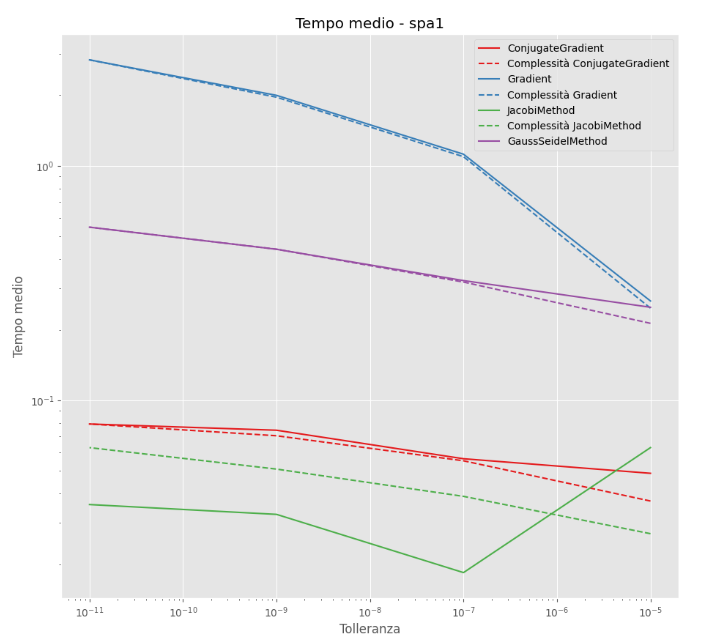
\includegraphics[width=\textwidth]{./../report/Progetto_1_bis/img/time_spa1.png}
        \caption{Matrice spa1}
        \label{fig:time_spa1}
    \end{subfigure}
    \hfill
    \begin{subfigure}{0.45\textwidth}
        \centering
        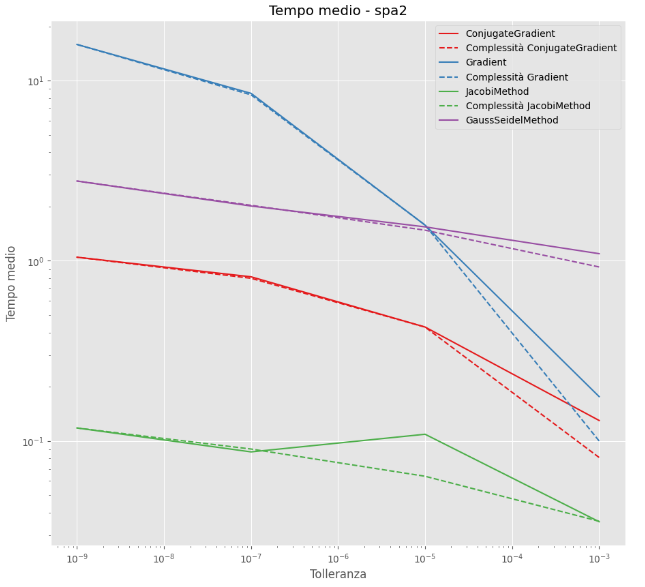
\includegraphics[width=\textwidth]{./../report/Progetto_1_bis/img/time_spa2.png}
        \caption{Matrice spa2}
        \label{fig:time_spa2}
    \end{subfigure}
    \hfill
    \begin{subfigure}{0.45\textwidth}
        \centering
        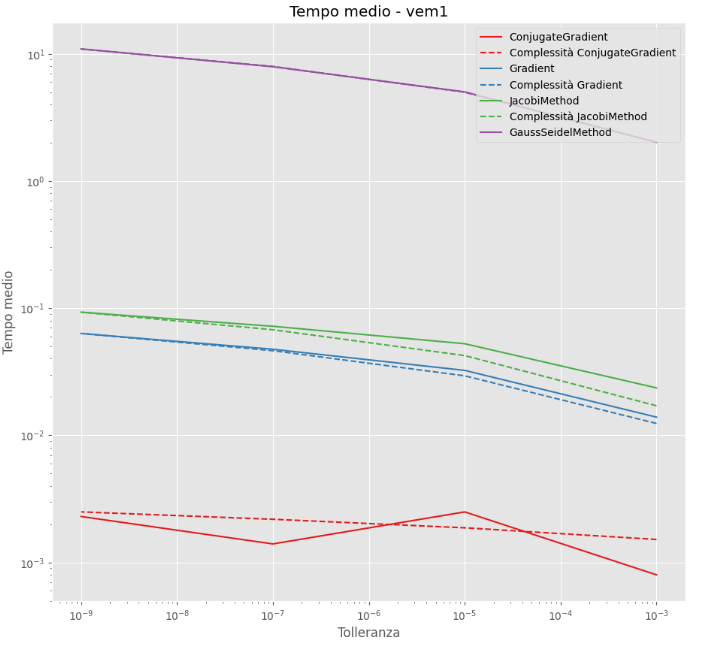
\includegraphics[width=\textwidth]{./../report/Progetto_1_bis/img/time_vem1.png}
        \caption{Matrice vem1}
        \label{fig:time_vem1}
    \end{subfigure}
    \hfill
    \begin{subfigure}{0.45\textwidth}
        \centering
        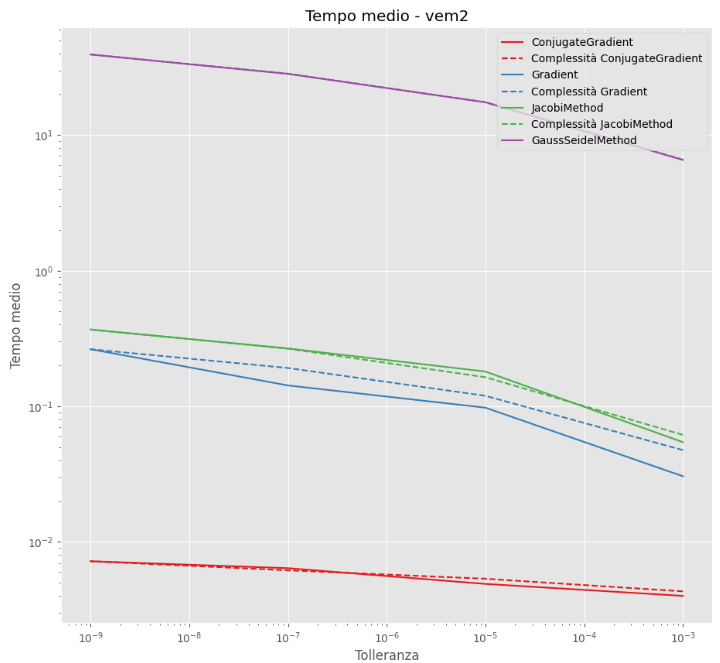
\includegraphics[width=\textwidth]{./../report/Progetto_1_bis/img/time_vem2.png}
        \caption{Matrice vem2}
        \label{fig:time_vem2}
    \end{subfigure}
    \caption{Tempi di esecuzione dei metodi iterativi}
    \label{fig:time}
\end{figure}

In questi grafici, si può osservare che per tutte le implementazioni il tempo di
esecuzione aumenta man mano che la tolleranza si avvicina allo zero. Questo
comportamento è prevedibile, poiché il numero di iterazioni necessarie per
raggiungere la tolleranza aumenta, come evidenziato nella tabella \ref{tab:iterazioni}.

\begin{table}[!ht]
    \centering
    \begin{subtable}[!ht]{1\textwidth}
        \centering
        \resizebox{\textwidth}{!}{\begin{tabular}{|c|c|c|c|c|c|c|c|c|c|c|c|c|c|c|c|c|}
                \textbf{matrice}    & \textbf{spa1}     & \textbf{spa1}     & \textbf{spa1} & \textbf{spa1} & \textbf{spa2}     & \textbf{spa2}     & \textbf{spa2} & \textbf{spa2} \\ \hline
                \textbf{metodo}     & ConjugateGradient & GaussSeidelMethod & Gradient      & JacobiMethod  & ConjugateGradient & GaussSeidelMethod & Gradient      & JacobiMethod  \\
                \textbf{tolleranza} & ~                 & ~                 & ~             & ~             & ~                 & ~                 & ~             & ~             \\
                \textbf{1e-05}      & 99                & 14                & 1332          & 149           & 90                & 8                 & 664           & 48            \\
                \textbf{1e-07}      & 147               & 21                & 5896          & 215           & 168               & 11                & 3508          & 68            \\
                \textbf{1e-09}      & 188               & 29                & 10576         & 281           & 220               & 15                & 6682          & 89            \\
                \textbf{1e-11}      & 211               & 36                & 15264         & 347           & 270               & 18                & 9894          & 110           \\
            \end{tabular}}
        \caption{Spa 1 e Spa 2}
        \label{tab:spa}
    \end{subtable}
    \hfill
    \begin{subtable}[!ht]{1\textwidth}
        \centering
        \resizebox{\textwidth}{!}{\begin{tabular}{|c|c|c|c|c|c|c|c|c|c|c|c|c|c|c|c|c|}
                \textbf{matrice}    & \textbf{vem1}     & \textbf{vem1}     & \textbf{vem1} & \textbf{vem1} & \textbf{vem2}     & \textbf{vem2}     & \textbf{vem2} & \textbf{vem2} \\ \hline
                \textbf{metodo}     & ConjugateGradient & GaussSeidelMethod & Gradient      & JacobiMethod  & ConjugateGradient & GaussSeidelMethod & Gradient      & JacobiMethod  \\
                \textbf{tolleranza} & ~                 & ~                 & ~             & ~             & ~                 & ~                 & ~             & ~             \\
                \textbf{1e-05}      & 42                & 940               & 1253          & 1875          & 52                & 1403              & 1873          & 2803          \\
                \textbf{1e-07}      & 49                & 1499              & 1975          & 2994          & 60                & 2278              & 3003          & 4552          \\
                \textbf{1e-09}      & 56                & 2059              & 2697          & 4113          & 70                & 3153              & 4131          & 6300          \\
                \textbf{1e-11}      & 62                & 2619              & 3421          & 5232          & 77                & 4027              & 5261          & 8049          \\
            \end{tabular}}
        \caption{Vem 1 e Vem 2}
        \label{tab:vem}
    \end{subtable}
    \caption{Iterazioni}
    \label{tab:iterazioni}
\end{table}
Inoltre, si nota che tutti i metodi tendono ad avere un andamento simile a quello
teorico.

Confrontando i vari metodi iterativi, il metodo di Gauß-Seidel risulta essere il
più lento per le matrici vem1 e vem2, nonostante il numero di iterazioni sia
inferiore rispetto ad altri metodi, come si può vedere nella tabella \ref{tab:iterazioni}.
Invece, per le matrici spa1 e spa2, il metodo che richiede più tempo è il metodo
del gradiente. Questo comportamento può essere attribuito al fatto che la convergenza
del metodo presenta un andamento a zig-zag. A supporto di questa ipotesi, si
osserva che il numero di condizionamento delle matrici spa1 e spa2 è molto elevato,
pari rispettivamente a 2048 e 1411. Pertanto, è plausibile che la combinazione
di un numero di condizionamento elevato e il punto di partenza scelto per il
metodo, ovvero il vettore nullo, conduca a un andamento a zig-zag nella convergenza.

\begin{table}[!ht]
    \centering
    \begin{subtable}[!ht]{1\textwidth}
        \centering
        \resizebox{\textwidth}{!}{\begin{tabular}{|c|c|c|c|c|c|c|c|c|c|c|c|c|c|c|c|c|}
                \textbf{matrice}    & \textbf{spa1}     & \textbf{spa1}     & \textbf{spa1} & \textbf{spa1} & \textbf{spa2}     & \textbf{spa2}     & \textbf{spa2} & \textbf{spa2} \\ \hline
                \textbf{metodo}     & ConjugateGradient & GaussSeidelMethod & Gradient      & JacobiMethod  & ConjugateGradient & GaussSeidelMethod & Gradient      & JacobiMethod  \\
                \textbf{tolleranza} & ~                 & ~                 & ~             & ~             & ~                 & ~                 & ~             & ~             \\
                \textbf{1e-05}      & 0.0488            & 0.2493            & 0.2652        & 0.0628        & 0.4021            & 1.4554            & 1.4882        & 0.0625        \\
                \textbf{1e-07}      & 0.0563            & 0.324             & 1.1214        & 0.0184        & 0.7542            & 2.0081            & 7.8689        & 0.0822        \\
                \textbf{1e-09}      & 0.0745            & 0.4407            & 1.999         & 0.0326        & 0.982             & 2.7038            & 14.9152       & 0.1058        \\
                \textbf{1e-11}      & 0.0792            & 0.5475            & 2.8326        & 0.0359        & 1.2048            & 3.1593            & 22.1536       & 0.1311        \\
            \end{tabular}}
        \caption{Spa 1 e Spa 2}
        \label{tab:spa_time}
    \end{subtable}
    \hfill
    \begin{subtable}[!ht]{1\textwidth}
        \centering
        \resizebox{\textwidth}{!}{\begin{tabular}{|c|c|c|c|c|c|c|c|c|c|c|c|c|c|c|c|c|}
                \textbf{matrice}    & \textbf{vem1}     & \textbf{vem1}     & \textbf{vem1} & \textbf{vem1} & \textbf{vem2}     & \textbf{vem2}     & \textbf{vem2} & \textbf{vem2} \\ \hline
                \textbf{metodo}     & ConjugateGradient & GaussSeidelMethod & Gradient      & JacobiMethod  & ConjugateGradient & GaussSeidelMethod & Gradient      & JacobiMethod  \\
                \textbf{tolleranza} & ~                 & ~                 & ~             & ~             & ~                 & ~                 & ~             & ~             \\
                \textbf{1e-05}      & 0.0018            & 4.7499            & 0.0324        & 0.0516        & 0.0051            & 16.681            & 0.0732        & 0.179         \\
                \textbf{1e-07}      & 0.0033            & 7.5831            & 0.0429        & 0.0707        & 0.0058            & 28.2671           & 0.1472        & 0.1964        \\
                \textbf{1e-09}      & 0.0023            & 10.3372           & 0.0594        & 0.0887        & 0.0053            & 45.1294           & 0.1924        & 0.337         \\
                \textbf{1e-11}      & 0.0042            & 13.1797           & 0.0773        & 0.1099        & 0.0076            & 59.9347           & 0.2712        & 0.4434        \\
            \end{tabular}}
        \caption{Vem 1 e Vem 2}
        \label{tab:vem_time}
    \end{subtable}
    \caption{Tempo medio di 10 esecuzioni}
    \label{tab:times}
\end{table}

Per quanto riguarda l'occupazione di memoria, i risultati ottenuti sono riportati
nelle figure \ref{fig:mem_spa1}, \ref{fig:mem_spa2}, \ref{fig:mem_vem1} e \ref{fig:mem_vem2}.

\begin{figure}[!ht]
    \centering
    \begin{subfigure}{0.45\textwidth}
        \centering
        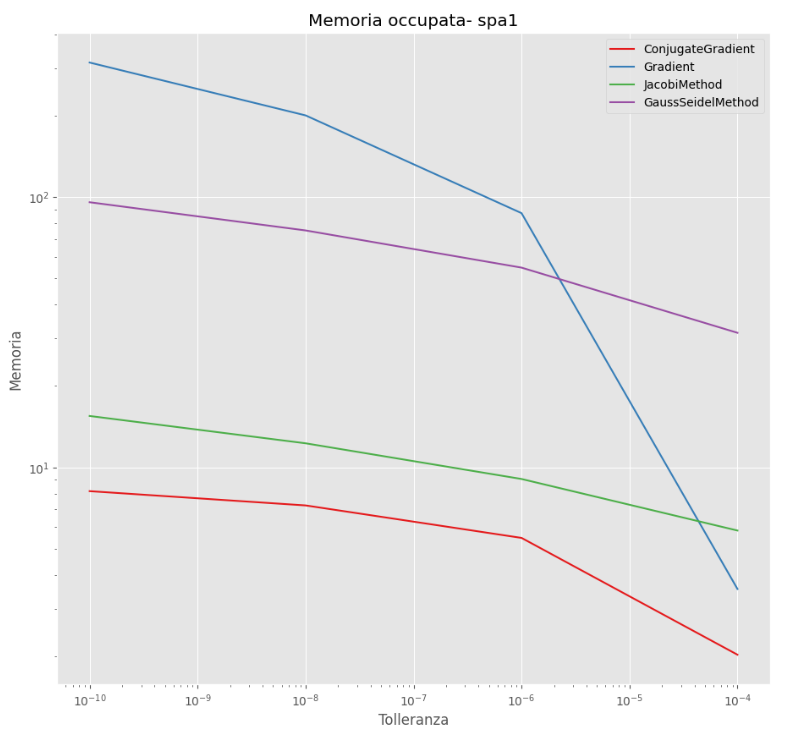
\includegraphics[width=\textwidth]{./../report/Progetto_1_bis/img/mem_spa1.png}
        \caption{Matrice spa1}
        \label{fig:mem_spa1}
    \end{subfigure}
    \begin{subfigure}{0.45\textwidth}
        \centering
        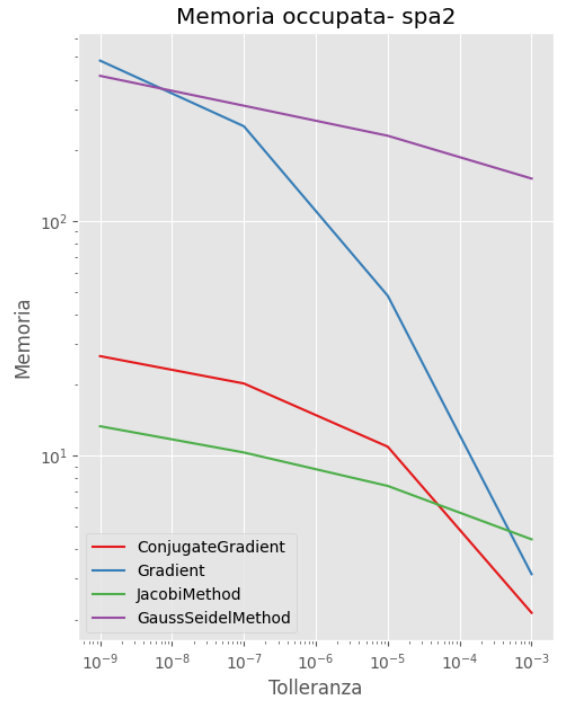
\includegraphics[width=\textwidth]{./../report/Progetto_1_bis/img/mem_spa2.png}
        \caption{Matrice spa2}
        \label{fig:mem_spa2}
    \end{subfigure}
    \begin{subfigure}{0.45\textwidth}
        \centering
        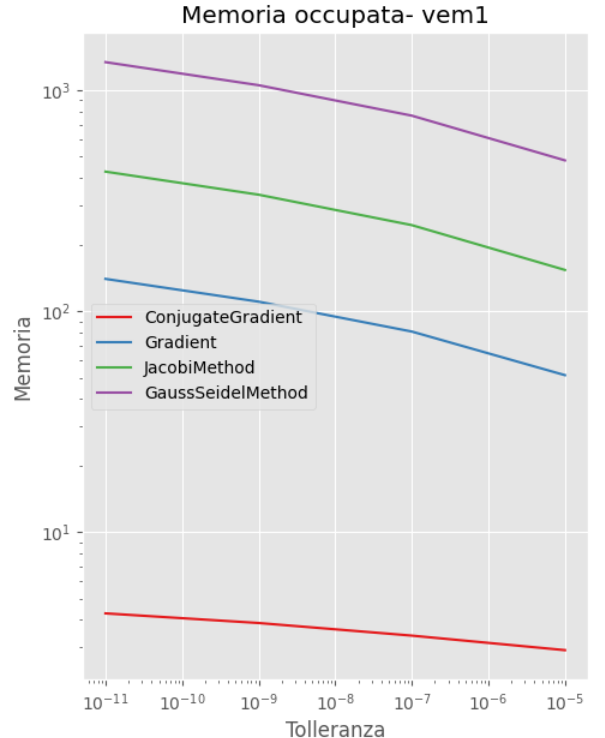
\includegraphics[width=\textwidth]{./../report/Progetto_1_bis/img/mem_vem1.png}
        \caption{Matrice vem1}
        \label{fig:mem_vem1}
    \end{subfigure}
    \begin{subfigure}{0.45\textwidth}
        \centering
        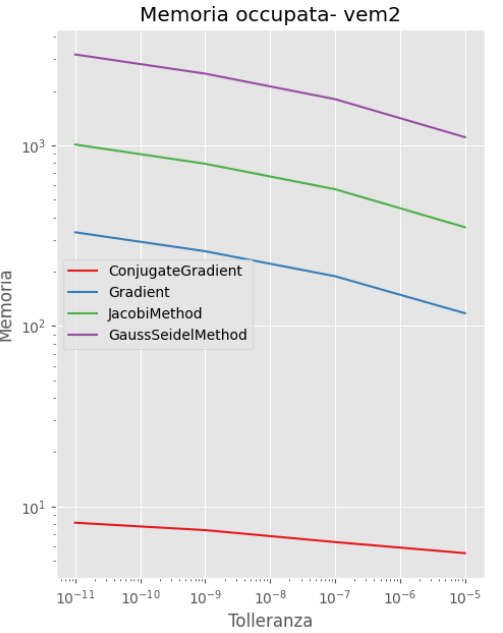
\includegraphics[width=\textwidth]{./../report/Progetto_1_bis/img/mem_vem2.png}
        \caption{Matrice vem2}
        \label{fig:mem_vem2}
    \end{subfigure}
    \caption{Memoria occupata dei metodi iterativi}
    \label{fig:memory}
\end{figure}

In questi grafici, possiamo notare lo spazio richiesto dai vari metodi cresce
all'aumentare del numero di iterazioni richieste per la convergenza. In generale
il metodo del gradiente coniugato richiede meno memoria rispetto agli altri metodi.


Infine, presentiamo i grafici che illustrano la variazione dell'errore medio in
funzione della tolleranza per ciascuna matrice, come mostrato nelle figure \ref{fig:error_spa1},
\ref{fig:error_spa2}, \ref{fig:error_vem1} e \ref{fig:error_vem2}.

\begin{figure}[!ht]
    \centering
    \begin{subfigure}{0.45\textwidth}
        \centering
        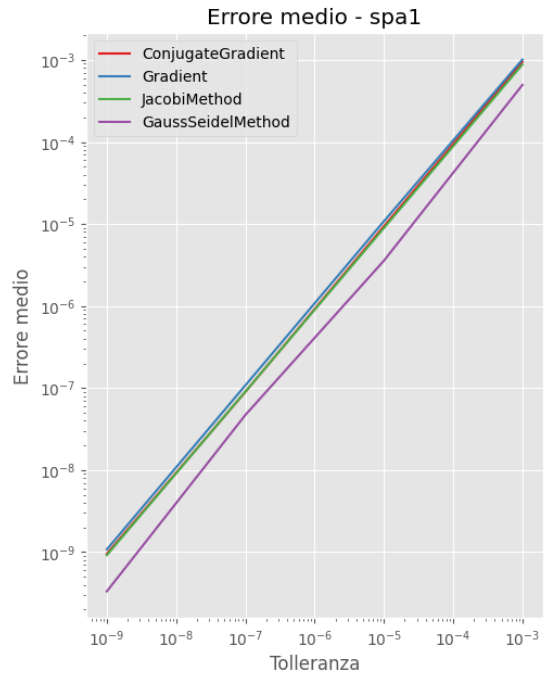
\includegraphics[width=\textwidth]{./../report/Progetto_1_bis/img/error_spa1.png}
        \caption{Matrice spa1}
        \label{fig:error_spa1}
    \end{subfigure}
    \begin{subfigure}{0.45\textwidth}
        \centering
        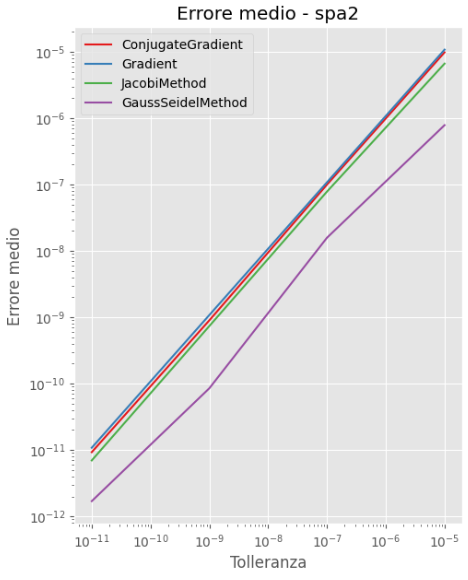
\includegraphics[width=\textwidth]{./../report/Progetto_1_bis/img/error_spa2.png}
        \caption{Matrice spa2}
        \label{fig:error_spa2}
    \end{subfigure}
    \begin{subfigure}{0.45\textwidth}
        \centering
        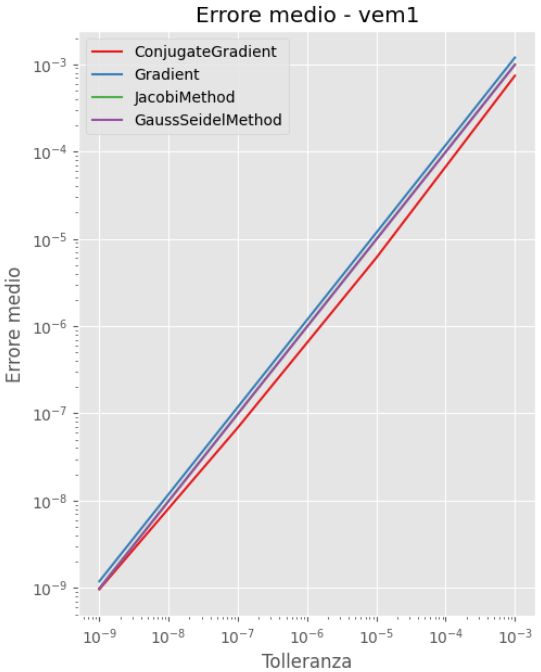
\includegraphics[width=\textwidth]{./../report/Progetto_1_bis/img/error_vem1.png}
        \caption{Matrice vem1}
        \label{fig:error_vem1}
    \end{subfigure}
    \begin{subfigure}{0.45\textwidth}
        \centering
        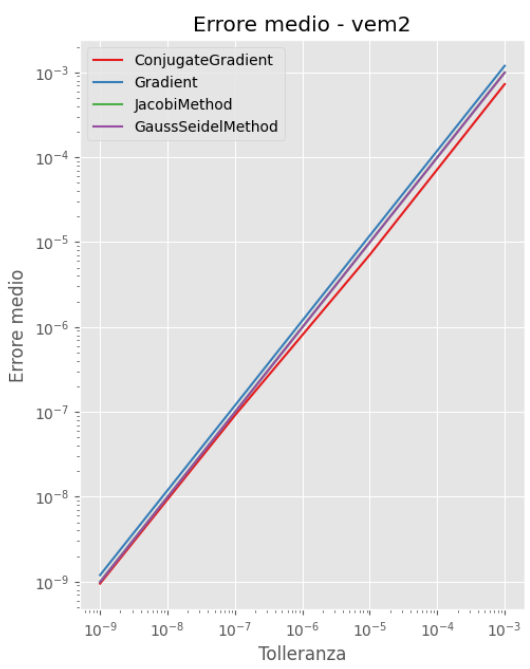
\includegraphics[width=\textwidth]{./../report/Progetto_1_bis/img/error_vem2.png}
        \caption{Matrice vem2}
        \label{fig:error_vem2}
    \end{subfigure}
    \caption{Errore dei metodi iterativi}
    \label{fig:error}
\end{figure}

In questi grafici possiamo osservare un andamento che decresce più la tolleranza
si avvicina a zero. Questo è legato al fatto che tutti i metodi implementati
convergono prima di raggiungere il numero di iterazioni massimo (20000). Inoltre,
non si riesce a notare una differenza significativa tra i metodi implementati.

\begin{table}[!ht]
    \centering
    \begin{subtable}[!ht]{1\textwidth}
        \centering
        \resizebox{\textwidth}{!}{    \begin{tabular}{|c|c|c|c|c|c|c|c|c|c|c|c|c|c|c|c|c|}
                \textbf{matrice}    & \textbf{spa1}     & \textbf{spa1}     & \textbf{spa1} & \textbf{spa1} & \textbf{spa2}     & \textbf{spa2}     & \textbf{spa2} & \textbf{spa2} \\ \hline
                \textbf{metodo}     & ConjugateGradient & GaussSeidelMethod & Gradient      & JacobiMethod  & ConjugateGradient & GaussSeidelMethod & Gradient      & JacobiMethod  \\
                \textbf{tolleranza} & ~                 & ~                 & ~             & ~             & ~                 & ~                 & ~             & ~             \\
                \textbf{1e-05}      & 4.056             & 43.1635           & 32.5122       & 7.4428        & 10.918            & 230.6839          & 48.0          & 7.4304        \\
                \textbf{1e-07}      & 6.0068            & 63.624            & 143.8008      & 10.6615       & 20.2967           & 309.7817          & 253.1776      & 10.3162       \\
                \textbf{1e-09}      & 7.673             & 87.0074           & 257.9179      & 13.8802       & 26.5492           & 415.2454          & 482.1626      & 13.3462       \\
                \textbf{1e-11}      & 8.6077            & 107.4679          & 372.2301      & 17.0989       & 32.5612           & 494.3431          & 713.8892      & 16.3763       \\
            \end{tabular}
        }
        \caption{Spa 1 e Spa 2}
        \label{tab:spa_mem}
    \end{subtable}
    \hfill
    \begin{subtable}[!ht]{1\textwidth}
        \centering
        \resizebox{\textwidth}{!}{\begin{tabular}{|c|c|c|c|c|c|c|c|c|c|c|c|c|c|c|c|c|}
                \textbf{matrice}    & \textbf{vem1}     & \textbf{vem1}     & \textbf{vem1} & \textbf{vem1} & \textbf{vem2}     & \textbf{vem2}     & \textbf{vem2} & \textbf{vem2} \\ \hline
                \textbf{metodo}     & ConjugateGradient & GaussSeidelMethod & Gradient      & JacobiMethod  & ConjugateGradient & GaussSeidelMethod & Gradient      & JacobiMethod  \\
                \textbf{tolleranza} & ~                 & ~                 & ~             & ~             & ~                 & ~                 & ~             & ~             \\
                \textbf{1e-05}      & 2.9174            & 481.4093          & 51.2975       & 153.6327      & 5.5209            & 1110.2653         & 117.5884      & 352.1476      \\
                \textbf{1e-07}      & 3.3945            & 767.5458          & 80.8244       & 245.1579      & 6.3574            & 1802.4533         & 188.4801      & 571.5982      \\
                \textbf{1e-09}      & 3.8716            & 1054.1941         & 110.3513      & 336.6832      & 7.403             & 2494.6413         & 259.2463      & 790.9232      \\
                \textbf{1e-11}      & 4.2806            & 1340.8424         & 139.96        & 428.2084      & 8.1349            & 3186.0382         & 330.138       & 1010.3737     \\
            \end{tabular}
        }
        \caption{Vem 1 e Vem 2}
        \label{tab:vem_mem}
    \end{subtable}
    \caption{Memoria utilizzata in MB}
    \label{tab:memory}
\end{table}


\begin{table}[!ht]
    \centering
    \begin{subtable}[!ht]{1\textwidth}
        \centering
        \resizebox{\textwidth}{!}{\begin{tabular}{|c|c|c|c|c|c|c|c|c|c|c|c|c|c|c|c|c|}
                \textbf{matrice}    & \textbf{spa1}     & \textbf{spa1}     & \textbf{spa1} & \textbf{spa1} & \textbf{spa2}     & \textbf{spa2}     & \textbf{spa2} & \textbf{spa2} \\ \hline
                \textbf{metodo}     & ConjugateGradient & GaussSeidelMethod & Gradient      & JacobiMethod  & ConjugateGradient & GaussSeidelMethod & Gradient      & JacobiMethod  \\
                \textbf{tolleranza} & ~                 & ~                 & ~             & ~             & ~                 & ~                 & ~             & ~             \\
                \textbf{1e-05}      & 9.348493e-06      & 3.565424e-06      & 1.0781389e-05 & 8.906615e-06  & 9.819377e-06      & 7.84728e-07       & 1.0782452e-05 & 6.639894e-06  \\
                \textbf{1e-07}      & 8.9837e-08        & 4.6975e-08        & 1.07936e-07   & 9.0406e-08    & 9.9676e-08        & 1.5783e-08        & 1.08016e-07   & 7.8238e-08    \\
                \textbf{1e-09}      & 9.53e-10          & 3.33e-10          & 1.08e-09      & 9.18e-10      & 9e-10             & 8.5e-11           & 1.082e-09     & 7.38e-10      \\
                \textbf{1e-11}      & 9e-12             & 4e-12             & 1.1e-11       & 9e-12         & 9e-12             & 2e-12             & 1.1e-11       & 7e-12         \\
            \end{tabular}}
        \caption{Spa 1 e Spa 2}
        \label{tab:spa_error}
    \end{subtable}
    \hfill
    \begin{subtable}[!ht]{1\textwidth}
        \centering
        \resizebox{\textwidth}{!}{\begin{tabular}{|c|c|c|c|c|c|c|c|c|c|c|c|c|c|c|c|c|}
                \textbf{matrice}    & \textbf{vem1}     & \textbf{vem1}     & \textbf{vem1} & \textbf{vem1} & \textbf{vem2}     & \textbf{vem2}     & \textbf{vem2} & \textbf{vem2} \\ \hline
                \textbf{metodo}     & ConjugateGradient & GaussSeidelMethod & Gradient      & JacobiMethod  & ConjugateGradient & GaussSeidelMethod & Gradient      & JacobiMethod  \\
                \textbf{tolleranza} & ~                 & ~                 & ~             & ~             & ~                 & ~                 & ~             & ~             \\
                \textbf{1e-05}      & 6.072082e-06      & 9.838476e-06      & 1.177959e-05  & 9.9321e-06    & 7.097885e-06      & 9.943094e-06      & 1.1934282e-05 & 9.951332e-06  \\
                \textbf{1e-07}      & 6.889e-08         & 9.8938e-08        & 1.18396e-07   & 9.9312e-08    & 9.1069e-08        & 9.9241e-08        & 1.18853e-07   & 9.9485e-08    \\
                \textbf{1e-09}      & 9.64e-10          & 9.87e-10          & 1.192e-09     & 9.93e-10      & 9.49e-10          & 9.91e-10          & 1.195e-09     & 9.97e-10      \\
                \textbf{1e-11}      & 4e-12             & 1e-11             & 1.2e-11       & 1e-11         & 6e-12             & 1e-11             & 1.2e-11       & 1e-11         \\
            \end{tabular}}
        \caption{Vem 1 e Vem 2}
        \label{tab:vem_error}
    \end{subtable}
    \caption{Errore medio dei metodi iterativi}
    \label{tab:erors}
\end{table}
